\documentclass[11pt]{article}

\usepackage[margin=2.4cm]{geometry}
\usepackage[T1]{fontenc}
\usepackage[utf8]{inputenc}
\usepackage{lmodern}
\usepackage{amsmath}
\usepackage{graphicx}
\usepackage{booktabs}
\usepackage{caption}
\usepackage[numbers,super,sort&compress]{natbib}
\usepackage{lineno}
\usepackage[colorlinks=true,allcolors=black]{hyperref}

\graphicspath{{figures/}}

\captionsetup{
  font=small,
  labelfont=bf,
  labelsep=period,
  justification=justified,
  singlelinecheck=false
}

\setlength{\parindent}{0pt}
\setlength{\parskip}{0.6em}
\linespread{1.15}

\newcommand{\Fovs}{F_{\mathrm{ov}}^{S}}
\newcommand{\degree}{$^\circ$}
\newcommand{\degS}{$^\circ$S}
\newcommand{\degN}{$^\circ$N}
\newcommand{\degW}{$^\circ$W}
\newcommand{\degE}{$^\circ$E}

\title{\vspace{-2.0cm}\bfseries The declining Atlantic overturning freshwater
transport at 34.5$^\circ$S is not explained by a declining overturning
transport}

\author{}
\date{}

\begin{document}

\maketitle
\thispagestyle{empty}
\vspace{-2.2cm}

\linenumbers

\section*{Abstract}

Freshwater transport by the overturning at the southern boundary of the
Atlantic, $\Fovs$, is the standard indicator of whether the salt-advection
feedback is self-reinforcing, and its recent decline in ocean reanalyses is
increasingly read as a warning that the overturning is weakening. We show that
it is not. Once the net throughflow is removed, $\Fovs$ factorises exactly as
$-T\,\Delta S/S_0$, with $T$ the northward-limb volume transport and $\Delta S$
the transport-weighted salinity difference between the limbs, both measured
directly from the section. At 34.5\degS{} $\Fovs$ changes at 36\% (ORAS5) and
52\% (GLORYS12V1) of its own magnitude per decade while $T$ changes at 2.6\%
and 0.6\%. The transport contributes 1\% to 18\% of the trend depending on how
the overturning is defined, in most configurations with the opposite sign, and
stays below 25\% in 97\% of all admissible epoch pairs in the two declining
products. What the decline
records instead is a widening limb salinity contrast, carried by the northward
limb; the EN4 observational analysis reproduces that asymmetry in a salinity field no
model integrates. The products disagree on the rest: ECCO-V4r4 has no trend to
attribute, and in ORAS5 the split between salinity and flow structure is not
resolved, with a third of the widening attributable to the flow.

\section*{Introduction}

The Atlantic meridional overturning circulation transports salt as well as
heat, and the resulting salt-advection feedback is the classical route to
multiple equilibria in this basin\cite{Stommel1961,Rahmstorf1996,Rahmstorf2002}.
The diagnostic used to test whether that feedback is self-reinforcing is
$\Fovs$, the freshwater transport carried by the overturning across the
southern boundary\cite{deVries2005,Huisman2010,Dijkstra2007}. When $\Fovs<0$
the overturning imports freshwater into the basin, so a weakening circulation
freshens the Atlantic and weakens it further; when $\Fovs>0$ the same
perturbation is damped. In box models and in coarse-resolution ocean models the
sign of $\Fovs$ separates a monostable from a bistable regime, and its value has
been used to argue that most climate models are biased towards the stable
side\cite{Weijer2019,Mecking2017,vanWestenDijkstra2024}.

That correspondence is not exact. Extended box models\cite{Cimatoribus2014}
and hysteresis experiments in a state-of-the-art coupled
model\cite{vanWestenDijkstra2023} show that the collapsed branch can persist
well outside the $\Fovs<0$ range, so the sign indicates where the freshwater
budget sits rather than proving that a second equilibrium exists. The
\emph{transient} behaviour of $\Fovs$ is a further step removed. $\Fovs$
reflects the salinity contrast between the limbs at the section, which responds
to North Atlantic anomalies only after they have been advected south, and an
AMOC collapse in a coupled model need not coincide with a minimum in
$\Fovs$\cite{vanWesten2025,Vanderborght2025}. Despite this, a declining $\Fovs$
is increasingly read as a physics-based early warning that the circulation is
weakening\cite{vanWesten2024,Zhu2020,Zhu2023}, and it is that inference we test.

The inference is not safe, for a reason visible in the definition. Write
$\Fovs$ as the product of an overturning transport and a salinity contrast.
Wherever $\Fovs<0$ the contrast is positive, so a weakening overturning
\emph{raises} $\Fovs$ rather than lowering it, and a falling $\Fovs$ cannot by
itself be evidence of a weakening circulation\cite{Vanderborght2025}. (The
argument applies only where $\Fovs<0$ throughout; ORAS5 has 7 years of 68 in
which it does not hold.) Whether the observed decline is carried by the
transport or by the salinity field is an empirical question, and it determines
how much of the recent literature on $\Fovs$ trends can be interpreted at all.

Answering it requires a factorisation whose two factors are separately
measurable. Defining the salinity contrast as $-S_0\Fovs/\Psi$ for some scalar
overturning strength $\Psi$ does not qualify: the second factor is then the
first divided out, it absorbs every change in the vertical structure of the
velocity as well as every change in salinity, and the resulting attribution is
fixed by algebra rather than by data. We therefore use the limb factorisation.
Removing the net section throughflow, which any transport-consistent estimate
of $\Fovs$ requires, forces the depth integral of the section velocity to
vanish, so the northward and southward limbs carry equal and opposite volume
transport $T$, and splitting the depth integral at the sign changes of the
velocity gives
\begin{equation}
\Fovs \;=\; -\frac{1}{S_0}\,T\,\Delta S,
\qquad \Delta S \;=\; S_{\uparrow}-S_{\downarrow},
\label{eq:factorisation}
\end{equation}
exactly and with no residual, where $S_{\uparrow}$ and $S_{\downarrow}$ are the
transport-weighted mean salinities of the northward and southward limbs.
Equation~\eqref{eq:factorisation} is not a linearisation and not a fit. Both
factors are computed directly from the section profile, $T$ is linear in the
velocity field and so carries none of the sampling bias of a streamfunction
maximum, and $\Delta S$ is a salinity difference that can be plotted, compared
between products, and in principle measured by hydrography.

We evaluate this at 34.5\degS{} in three ocean reanalyses recomputed here from
monthly fields, ORAS5, GLORYS12V1 and ECCO-V4r4, spanning two ocean models and
three assimilation methods, and we ask what the answer implies for the
interpretation of CMIP6 freshwater transport biases.

\section*{Results}

\subsection*{A negative freshwater transport, and the two factors that set it}

Recomputed from monthly fields on the contiguous Atlantic section
(Methods), the record-mean $\Fovs$ at 34.5\degS{} is negative in all three
reanalyses (Fig.~\ref{fig:sign}a,b): $-0.038$~Sv in ORAS5 over 1958--2025,
$-0.084$~Sv in GLORYS12V1 over 1993--2025 and $-0.132$~Sv in ECCO-V4r4 over
1992--2017. The sign is not marginal. It holds in 61 of 68 annual means in
ORAS5, 32 of 33 in GLORYS12V1 and 26 of 26 in ECCO, and the 95\% circular
block-bootstrap interval excludes zero in every product at every block length
from 2 to 20 years, so the result does not depend on that choice. Because a
mean over a trending record is not an estimate of any well-defined population
quantity, we also give the most recent decade, which is the quantity a reader
interested in the present state should use: $-0.088$~[$-0.094$, $-0.080$]~Sv in
ORAS5 over 2016--2025, $-0.132$~[$-0.141$, $-0.121$] in GLORYS12V1 and
$-0.128$~[$-0.136$, $-0.119$] in ECCO over 2008--2017.

A fourth product, SODA 3.15.2, gives $-0.009$~Sv with an interval that includes
zero, but we do not count it either way. The archive we can obtain provides
annual rather than monthly fields, and $\Fovs$ is bilinear in velocity and
salinity, so forming it from annual means discards the within-year covariance.
Measured directly in ECCO, where both routes are available, that omission shifts
$\Fovs$ by $+0.012$~Sv, larger in magnitude than SODA's entire record mean. The
same test gives $+0.000$~Sv in ORAS5 and $-0.001$~Sv in GLORYS12V1, so the bias
is product-dependent and small in the two eddy-permitting products. SODA can
neither support nor refute the sign, and we say so rather than counting it.

The magnitudes span a factor of three across the three products, which is
larger than any within-product interval. The reanalyses differ more about how
much freshwater the overturning carries than about which way it carries it, and
only the second statement is robust.

Equation~\eqref{eq:factorisation} splits each of these numbers into a transport
and a salinity contrast. The northward limb carries 18.7~Sv in ORAS5, 21.3~Sv
in GLORYS12V1 and 14.6~Sv in ECCO, against limb salinity contrasts of $+0.068$,
$+0.136$ and $+0.307$~PSU. (The factorisation is exact year by year, so the
product of the record means differs slightly from the mean of the products, by
6\% in ORAS5.) Almost the entire three-product spread in $\Fovs$ is in
$\Delta S$, which varies by a factor of 4.5, not in $T$, which varies by a
factor of 1.5. Whatever the reanalyses constrain at this section, it is the
transport far better than the salinity structure.

\subsection*{The decline outruns the transport by an order of magnitude}

ORAS5 and GLORYS12V1 both decline over their own records, by $-1.37$~mSv per
year ($p<10^{-4}$, $N_{\text{eff}}=23.7$) and $-4.36$~mSv per year
($p=0.017$, $N_{\text{eff}}=7.2$). ECCO does not decline at all
($+0.11$~mSv per year, $p=0.76$, $N_{\text{eff}}=23.1$, minimum detectable
trend 0.75~mSv per year). Over the 1993--2017 window all three share, no
product has a significant \emph{$\Fovs$} trend, but that is a statement about
power rather than about the ocean: the smallest trend those 25 years could have
resolved is 1.3~mSv per year in ORAS5 and 7.1 in GLORYS12V1, and the GLORYS12V1
point estimate over the common window ($-4.76$) is larger in magnitude than over
its own record. The northward-limb transport behaves differently over that same
window, and in the opposite direction to the paper's framing: it declines in all
three products, by $-0.97$~Sv per decade in ORAS5 ($p=0.052$,
$N_{\text{eff}}=10.1$), $-0.75$ in GLORYS12V1 ($p=0.036$, $N_{\text{eff}}=14.3$)
and $-0.35$ in ECCO ($p=0.062$, $N_{\text{eff}}=21.3$). Over the one window in
which the three products are directly comparable it is the transport, not
$\Fovs$, that has the near-significant trends.

The cleanest statement of the result needs no ratio at all. Expressed as
fractional rates, $\Fovs$ is changing at $-36$\% of its own magnitude per decade
in ORAS5 and $-52$\% in GLORYS12V1, while the transport that carries it changes
at $-2.6$\% and $-0.6$\% per decade. Over the Argo era the same comparison gives
$-35$\% against $-0.7$\% and $-20$\% against $+0.8$\%. In those windows the two quantities are
changing at rates that differ by between one and two orders of magnitude, which
is the argument in its simplest form and is free of any denominator that might
approach zero. The separation is not uniform across every window: over the
common 1993--2017 window, where the $\Fovs$ trend is not resolvable and the
transport trend nearly is, the ORAS5 ratio narrows to 2.5. Across the four
windows we examine, the transport rate is between 1\% and 132\% of the $\Fovs$
rate in the two declining products. The wide end comes entirely from windows in
which the $\Fovs$ trend is not resolvable: 40\% from the common window in
ORAS5 and 132\% from the eleven-year clean window in GLORYS12V1, where the
$\Fovs$ trend has the wrong sign and $p=0.79$. Over the windows in which the
denominator is resolvable the range is 1\% to 7\%.

Splitting the trend by equation~\eqref{eq:factorisation} puts numbers on it
(Fig.~\ref{fig:attribution}b). In ORAS5 the total is $-1.37$~mSv per year, of
which the transport term contributes $+0.09$ [$+0.06$, $+0.13$], the salinity
term $-1.46$ [$-1.77$, $-1.14$] and a covariance residual $+0.002$, 3\% of the
transport term. In GLORYS12V1 the total is $-4.36$, the transport term $+0.05$
[$-0.12$, $+0.21$], the salinity term $-4.36$ [$-5.78$, $-2.94$] and the
residual $-0.05$, which is 108\% of the transport term and larger than it. The
transport share of the trend is 0.068 [0.046, 0.094] in ORAS5 and 0.012
[0.001, 0.051] in GLORYS12V1; assigning the residual entirely to the transport
instead of dropping it moves the GLORYS12V1 share to 0.001 and flips its sign, so for that product the honest statement is that the transport
contribution is not distinguishable from zero rather than that it is
positive. The transport term opposes the total with probability 1.00 in ORAS5
over its own record but only 0.73 in GLORYS12V1, and 0.36 in GLORYS12V1 over
the Argo era, where its point estimate ($-0.09$~mSv per year) has the same sign
as the total. The magnitude claim is robust; the sign claim is not universal
and we do not make it universal.

What the salinity term represents is unusually specific
(Fig.~\ref{fig:mechanism}a). The contrast $\Delta S$ widens because the
northward limb becomes saltier while the southward limb does not change.
$S_{\uparrow}$ rises by $+0.025$~PSU per decade in ORAS5 ($p<10^{-4}$,
$N_{\text{eff}}=24.2$) and $+0.071$ in GLORYS12V1 ($p=0.017$,
$N_{\text{eff}}=6.9$, which is under five degrees of freedom and should be read
accordingly), whereas $S_{\downarrow}$ changes by $-0.002$ ($p=0.06$) and
$-0.001$ ($p=0.24$) over the same records. The southward limb is not
uniformly flat: over the matched 1993--2017 window the ORAS5 value is
$-0.003$ and does reach significance ($p=0.006$). The asymmetry rests on
magnitude, $S_{\uparrow}$ moving six times faster, rather than on
$S_{\downarrow}$ being exactly stationary. Over the Argo era the two products converge, to $+0.051$
($p=0.009$) and $+0.035$ ($p=0.005$); note that this is a rise for ORAS5 and a
halving for GLORYS12V1, so the agreement improves while the GLORYS12V1 rate
falls. Over the matched 1993--2017 window neither is individually significant
($+0.019$, $p=0.11$, $N_{\text{eff}}=15.8$; $+0.083$, $p=0.10$,
$N_{\text{eff}}=5.2$) and they differ by a factor of four.

The depth-resolved salinity trends behind these numbers disagree far more than
the limb-weighted quantities do (Fig.~\ref{fig:mechanism}b). Through the upper
500~m GLORYS12V1 trends at $+0.10$ to $+0.13$~PSU per decade against a
layer-mean $+0.009$ in ORAS5, which crosses zero near 200~m, so the two differ
by more than an order of magnitude and are jointly significant over only a
narrow band near 600~m. That the transport-weighted limb
salinities agree to within a factor of 2.3 over 1993--2025 while the raw profiles
disagree by more than ten is an argument for weighting by the transport that
actually carries the salt rather than by depth.

ECCO is the counterexample, and against GLORYS12V1 it is a real one rather than
a lack of power. Its limb salinities are flat ($+0.005$~PSU per decade,
$p=0.55$, $N_{\text{eff}}=14.9$). On the matched 1993--2017 window its minimum
detectable $S_{\uparrow}$ trend is 0.020~PSU per decade, well below the
GLORYS12V1 rate of $+0.083$ over the same years, so ECCO could have resolved
that salinification and did not. Against ORAS5 the comparison is inconclusive:
the ORAS5 common-window rate, $+0.019$~PSU per decade, is itself below ECCO's
detection limit.

\subsection*{Is the widening contrast a water mass, or a redistribution?}

$\Delta S$ is transport-weighted, so it changes if the salinity field changes,
and also if transport is redistributed in depth at a completely fixed salinity
field. The two have to be separated before the change can be called a water-mass
signal. Recomputing $\Delta S$ with the salinity profile frozen at its record
mean, and again with the velocity profile frozen, does that at the full vertical
resolution of the section, and the answer differs between products.

In GLORYS12V1 the change is almost all salinity: the salinity-only trend is
$+0.068$~PSU per decade ($p=0.048$, $N_{\text{eff}}=4.8$) against a full trend
of $+0.072$, a share of 0.94, and the velocity-only trend is $+0.007$, not
significant and close to its own detection limit ($p=0.22$,
$N_{\text{eff}}=22.0$, detection limit 0.011).
In ORAS5 the partition is not resolved. The point estimates give a salinity
share of 0.66 and a velocity share of 0.39, so roughly a third of the widening
is a change in the vertical structure of the flow rather than in the water
masses. But the salinity-only series is so persistent (lag-1 autocorrelation
0.93) that its effective sample size falls to the floor of 3 imposed by the
significance test, and the smallest trend it could have resolved is
0.199~PSU per decade, eleven times the estimate itself. Its $p=0.45$ therefore
carries no information. The velocity-only term is the resolvable one
($+0.011$~PSU per decade, $p=0.0002$, $N_{\text{eff}}=31.9$, detection limit
0.005), so what can be said of ORAS5 is that a flow-structure contribution is
definitely present, not that the salinity contribution is absent. In GLORYS12V1
the salinity-only estimate also sits close to its own detection limit
($+0.068$ against 0.066, $N_{\text{eff}}=4.8$). In ECCO neither term is
resolvable ($-0.006$, detection limit 0.010; $+0.009$, detection limit 0.027)
and the full trend is indistinguishable from zero. The two shares sum
to slightly more than one because the split leaves a small covariance residual,
$-5$\% in ORAS5 and $-4$\% in GLORYS12V1.

The coarse component of that redistribution can be isolated further. The limbs
are defined by the sign of the section velocity, and that sign changes more than
once: besides the upper cell there is a northward abyssal limb of Antarctic
Bottom Water carrying 3.8~Sv in ORAS5, 4.8 in GLORYS12V1 and 2.2 in ECCO, that
is 20\%, 23\% and 15\% of the northward limb, and fresher than the upper cell by 0.21 to
0.49~PSU (Extended Data Fig.~2a,c). Writing $S_{\uparrow}=\sum_i w_i S_i$ over
the sub-limbs and holding either the weights or the sub-limb salinities at their
record means splits it. The partition term is small and of the opposite sign to
the total in both declining products: in ORAS5 the change in $S_{\uparrow}$ of
$+0.027$~PSU per decade is a water-mass term of $+0.030$ and a partition term of
$-0.003$, a share of 0.12; in GLORYS12V1, $+0.072$ splits into $+0.073$ and
$-0.002$, a share of 0.03. So the upper-to-abyssal redistribution is not what
drives the ORAS5 velocity term; that lives within the upper limb.

ECCO is the one product in which the coarse redistribution is significant and
active. Its upper-cell transport falls at $-0.60$~Sv per decade ($p=0.011$)
while its abyssal limb rises at $+0.36$ ($p=0.041$), and its upper-cell salinity
rises at $+0.022$~PSU per decade ($p=0.025$), the same sign as the other two
products. That last $p$ is basis-dependent: identifying the sub-limbs on
annual-mean profiles instead gives $+0.018$ and $p=0.18$, so the ECCO
cancellation is suggestive rather than established.
ECCO's flat whole-limb salinity is therefore the sum of a positive water-mass
term and a redistribution that cancels it, not an absence of change, and the
confound this section exists to test is demonstrably real even though it is not
what dominates elsewhere.

Excluding the abyssal cell altogether points the same way as the sub-limb split.
Truncating the section at the deep zero crossing and re-applying the throughflow
removal within the truncated layer, so the factorisation is again exact, gives
upper-cell $S_{\uparrow}$ trends of $+0.033$~PSU per decade in ORAS5
($p<10^{-4}$) and $+0.086$ in GLORYS12V1 ($p=0.033$), larger than the whole-limb
values, with transport shares of 0.112 and 0.019.

\subsection*{An observation-only test}

The claim that the northward limb is becoming saltier can be tested in a
salinity field that no ocean model integrates forward. We take EN4.2.2, an
objective analysis of profile observations, hold the velocity structure frozen
at each reanalysis record-mean profile, and let only the observed salinity vary
over 2005--2024 (Methods). Any trend is then a trend in observed water masses
under a fixed circulation. EN4 is on whole-degree latitudes, and we use the
34\degS{} row: the 35\degS{} row lies south of Cape Agulhas, where Africa no
longer closes the basin and a contiguous section runs into the Indian Ocean.

The limb asymmetry is reproduced, and more clearly than in the reanalyses'
own statistics. $S_{\uparrow}$ rises at $+0.026$~PSU per decade ($p=0.0005$)
under the ORAS5 velocity structure and $+0.028$ ($p=0.0003$) under the
GLORYS12V1 structure, while $S_{\downarrow}$ is flat in both ($+0.002$,
$p=0.09$), and the contrast widens at $+0.024$ to $+0.026$~PSU per decade
($p=0.0001$). The sign, the limb asymmetry and the significance therefore
survive in a salinity field that no assimilating model has touched.

The observed salinity field also supplies an observational estimate of $\Fovs$
itself. Combined with the frozen transport it gives $-0.080$~Sv under the ORAS5
velocity structure and $-0.128$~Sv under the GLORYS12V1 structure, both firmly
negative. This is not an independent measurement, since the transport is taken
from the reanalyses, but it shows the negative sign does not depend on the
reanalysis salinity fields. It also sharpens the disagreement about magnitude:
under ORAS5's own velocity structure the observed salinity field returns
$-0.080$~Sv against ORAS5's own $-0.038$~Sv, because EN4's limb contrast at this
section is 0.160~PSU against ORAS5's 0.068.

The rate is a different matter. Over the identical 2005--2024 window the
reanalyses give $S_{\uparrow}$ trends of $+0.056$ (ORAS5) and $+0.035$
(GLORYS12V1)~PSU per decade, against $+0.026$ and $+0.028$ from the
observations. ORAS5 runs about twice the observation-only rate while GLORYS12V1
is within 30\% of it. Part of that gap is expected by construction, since EN4
relaxes towards climatology where profiles are sparse and the core Argo array
does not sample below 2000~m, so the observation-only estimate is a lower bound.
The direction is robust; the ORAS5 rate should not be taken at face value.

\subsection*{The attribution does not depend on the choices we made}

\emph{Epoch selection.} Rather than quoting hand-picked epochs, we evaluate the
symmetric decomposition of equation~\eqref{eq:factorisation} for every
non-overlapping early and late epoch pair each record supports, at epoch lengths
of 10, 13 and 15 years: 2901 usable pairs in ORAS5 and 151 in GLORYS12V1. These
are not independent samples, and we treat them as a sensitivity analysis over
window choice rather than as evidence from a large sample. The median transport
share is 0.075 in ORAS5 and 0.038 in GLORYS12V1, the 95th percentile is 0.219
and 0.088, the maximum is 0.90 and 0.12, and the share is below 0.25 in 96.8\%
and 100\% of pairs (Fig.~\ref{fig:attribution}c). The transport term opposes the
total in 96.8\% and 94.7\% of pairs. The symmetric form uses the mean of the two
epochs as its coefficient, so it has no cross term and does not depend on which
epoch is the base point; the early-base and late-base conventions bracket it,
with median shares of 0.012 and 0.141 in ORAS5.

\emph{The definition of overturning strength.} Substituting the depth-space
streamfunction maximum for the limb transport, either integrated from the
surface or with the integration restarted at 250~m to exclude the wind-driven
surface cell, changes the mean overturning strength substantially, from 18.7 to
14.6 to 8.6~Sv in ORAS5, and raises the share to 0.111 [0.076, 0.151] and 0.183
[0.137, 0.240]; in GLORYS12V1 it becomes 0.014 and 0.040. The share therefore
rises monotonically as the definition of the overturning narrows, by a factor of
2.4 across the three definitions computed on this common basis (0.076, 0.111 and
0.183 for ORAS5), and the full range across every test in which the share is
identified, excluding the census tail, is 1\% to 18\% with individual intervals
reaching 27\%; the two largest values with a resolvable denominator are
0.18 over 1993--2025 in ORAS5 and 0.183 for the 250~m streamfunction definition
over its full record. It remains a
minority contribution throughout, but it is not definition-independent, and we
note that the factorisation we advocate gives a smaller share than the
construction it replaces.

\emph{The observing system.} The salinity field at 34.5\degS{} was barely
constrained before Argo, so we repeat everything from 2004 onwards. The
GLORYS12V1 decline survives ($-2.28$~mSv per year, $p=0.038$) and its transport
share rises, to 0.038 [0.004, 0.268], while remaining a minority. GLORYS12V1 has no documented stream join, but its record
crosses the Argo transition, and applying the same level-shift model at 2004
shows that most of its signal is a step rather than a trend: the residual trend
falls to $-1.90\pm1.07$~mSv per year ($p=0.098$, not significant) against a step
of $-0.061\pm0.022$~Sv ($p=0.014$), and the limb contrast behaves the same way
($+0.029\pm0.015$~PSU per decade, $p=0.071$, against a step of
$+0.105\pm0.031$, $p=0.004$). The attribution is unaffected, the step-adjusted
transport share being 0.045 and the step-adjusted fractional rate 23\% per
decade rather than 52\%, but the GLORYS12V1 \emph{decline} is a level shift
at the arrival of Argo and should not be read as a trend.

ORAS5 is also a splice, the consolidated
reanalysis to 2014 and the operational stream thereafter, and here too the test
is weaker than it looks. Fitting a trend together with a level shift at 2015 gives, over
the full record, a step in $\Fovs$ of $-0.017\pm0.011$~Sv ($p=0.15$); the
corresponding step in the limb salinity is larger relative to its own signal and
is significant, $+0.038\pm0.017$~PSU ($p=0.029$), and allowing for it reduces
the $S_{\uparrow}$ trend from $+0.025$ to $+0.020$~PSU per decade. Refitting over
2004--2025 alone gives a trend of $-1.36\pm1.53$~mSv per year that is not
significant, against $-2.46$ when the step is ignored. The ORAS5 Argo-era decline does not survive fitting the splice. Over the full record the step-adjusted trend is
$-1.17\pm0.21$~mSv per year ($p<10^{-4}$), essentially identical to the
consolidated-stream-only value of $-1.17$ ($p=5\times10^{-5}$), whose transport
share is 0.050 [0.024, 0.083]. So roughly 15\% of the raw ORAS5 full-record decline is
the splice, the decline survives correcting for it over the full record, and the
attribution is unaffected; but the 22-year Argo window alone cannot separate the
two.

\emph{The one window with neither confound.} 2004--2014 is inside the Argo era
and inside the ORAS5 consolidated stream at once. It is short, and it settles
nothing: over it the ORAS5 fractional-rate ratio is 0.152 with an $\Fovs$ trend that
is not resolvable, and GLORYS12V1 gives an $\Fovs$ trend of the opposite sign
($+7$\% per decade, $p=0.79$) against a transport falling at $-9$\% per decade
($p=0.0005$), so its fractional-rate ratio is 1.32; ECCO gives 0.30. Eleven years cannot
separate these quantities, and we report the window rather than omit it because
it is the only one that satisfies both homogeneity conditions.

\emph{The removal of the net transport.} Taking the net section transport out in
proportion to $|V|$, so that it is removed where the flow is rather than
uniformly over the area, changes $T$ by less than 0.6\% and leaves the
attribution intact: the transport share becomes 0.078 in ORAS5 and 0.012 in
GLORYS12V1, against 0.068 and 0.012 for the scheme used throughout.

\emph{The window.} Over 1993--2025, the longest window the two eddy-permitting
products share, both limb-salinity trends are resolvable ($+0.031$~PSU per
decade, $p=0.004$, in ORAS5 and $+0.071$, $p=0.017$, in GLORYS12V1, a factor of
2.3 apart rather than the factor of four over the shorter three-product window).
The ORAS5 transport share on that window is 0.180, and still a minority.

\emph{The section.} Recomputing the whole diagnostic at 25, 28, 30, 32 and
34.5\degS{} over the matched 1993--2025 window (Fig.~\ref{fig:sign}c), the
record mean is negative at every latitude in both products, and its interval
excludes zero everywhere except ORAS5 at 25\degS{} ($-0.004$~Sv). The magnitude
varies by a factor of 22 in ORAS5 across the full band and by 1.5 in
GLORYS12V1, and at 25\degS{} the two products disagree by a factor of 22, a
larger disagreement than any we report at 34.5\degS{}. (The two factors, 22.5
and 22.6, are close by coincidence.) Excluding 25\degS{}, the
ORAS5 range narrows to a factor of two. The negative sign is established in
ORAS5 only poleward of about 28\degS{}. We use 34.5\degS{} because that is
where the observing array sits and where the diagnostic is defined.

Two further quantities bound what the diagnostic means. The net volume
transport across the section is $-1.2$~Sv in ORAS5, $-1.2$ in GLORYS12V1 and
$-1.0$ in ECCO, and removing it in order to define an overturning component
shifts $\Fovs$ by $+0.009$, $+0.008$ and $+0.007$~Sv. Separately, the
overturning is not the only freshwater carrier at this section: the azonal
component is $+0.306$~Sv in ORAS5, $+0.304$ in GLORYS12V1 and $+0.155$ in ECCO,
opposite in sign to $\Fovs$ and, in the eddy-permitting products, several times
larger. Its trend is also opposite and, over each product's own record,
significant: $+1.84$~mSv per year in ORAS5 ($p=0.0002$, $N_{\text{eff}}=21.8$)
and $+6.68$ in GLORYS12V1 ($p=0.049$, $N_{\text{eff}}=8.5$, so marginal on few
effective degrees of freedom), both larger in magnitude than the $\Fovs$ trends
they accompany, against $+0.19$ ($p=0.95$) in ECCO, where the
detection limit is 14~mSv per year and the null is uninformative. The total freshwater transport
across 34.5\degS{} is therefore not moving the way $\Fovs$ alone implies, and a
reader assessing whether the basin is moving deeper into the self-reinforcing
regime must weigh both. $\Fovs$ is a stability diagnostic defined on the
overturning component; it is not the freshwater budget of the basin.

\subsection*{Implications for climate models}

CMIP6 historical simulations sit on the other side of zero, but not by a
majority that can be tested. Over 1950--1980, 16 of 25 models have a positive
mean $\Fovs$ at 34.5\degS{}, with a median of $+0.053$~Sv against a range of
$-0.205$ to $+0.405$~Sv (Fig.~\ref{fig:models}a). That count is not
distinguishable from a coin flip (binomial $p=0.23$), and taking one member per
model family leaves 18 independent models of which 10 are positive
($p=0.81$), or 9 if the other member of the one internally inconsistent family
is chosen ($p=1.00$). The defensible statement is about location rather than
majority: the model median is $+0.053$~Sv while all three recomputed
observational estimates lie between $-0.038$ and $-0.132$~Sv, below 72\%, 80\%
and 88\% of the models respectively. This confirms a bias documented
previously\cite{Mecking2017,vanWestenDijkstra2024,Weijer2019} and benchmarks it
against three consistently computed estimates; it does not discover it. The
model means are over 1950--1980 while the reanalyses cover modern decades, and
since ORAS5 declines by 1.37~mSv per year the two windows are not equivalent;
the comparison should be read as a statement about a persistent model offset,
not as a like-for-like difference of contemporaneous states.

Whether that bias matters for projected rates is a separate question, and the
test that has been used to answer it has no power. Correlating model mean
$\Fovs$ against a 19-year overturning trend at 26.5\degN{} over 2005--2023
gives $r=-0.04$ ($p=0.88$) across 16 models, but the smallest correlation that
sample could reach significance with is $|r|=0.50$, and 19-year overturning
trends within a single model's large ensemble already span $-3.5$ to
$+2.4$~Sv per decade across 50 members of MPI-ESM1-2-LR. A null from such a test
is guaranteed by internal variability whatever the forced relationship. The
counting statistic behaves the same way: 2 of 6 models with negative $\Fovs$
weaken faster than GLORYS12V1 (whose own rate at 26.5\degN{} is $-0.70$~Sv per
decade) against 6 of 10 with positive $\Fovs$, a Fisher exact $p$ of 0.61, with the same counts against the RAPID rate.

Repeating the test on the forced response, where the signal is large, remains
negative but is now informative. Across 21 models with historical plus ssp585
projections to 2100, mean $\Fovs$ and the overturning change from 1850--1900 to
2081--2100 give $r=-0.20$ ($p=0.40$, 95\% CI $-0.58$ to $+0.26$) against a
smallest reachable $|r|$ of 0.43 (Fig.~\ref{fig:models}b); on fractional rather
than absolute change $r=+0.30$ ($p=0.18$). Leaving out one model at a time
moves the first between $-0.41$ and $-0.05$ and the second between $+0.06$ and
$+0.45$, so neither is stable.

The reason the two have opposite signs is itself the one significant result in
this comparison. Model mean $\Fovs$ and the pre-industrial overturning strength
are strongly correlated ($r=+0.73$, $p=1.5\times10^{-4}$, 95\% CI $+0.44$ to
$+0.89$, $n=21$): models with a stronger overturning carry a more positive
$\Fovs$, which is what equation~\eqref{eq:factorisation} predicts given that
these models mostly carry $\Delta S<0$. Absolute overturning change is
mechanically tied to the base state while fractional change is not, which is
why the two rate tests disagree in sign. It also suggests that the CMIP6
$\Fovs$ bias is in part a symptom of the overturning strength bias rather than
an independent error in the freshwater budget.

The observed rate is itself weakly constrained. Over 2005--2023 the RAPID array
gives $-0.89$~Sv per decade at 26.5\degN{}, with an unadjusted $p$ of 0.093
that becomes 0.21 once the effective sample size is accounted for
($N_{\text{eff}}=11.9$). The direct observations do not yet establish a
significant decline over the era in which the reanalyses are best
constrained\cite{Jackson2024,Terhaar2025}.

\clearpage

\begin{figure}[t]
  \centering
  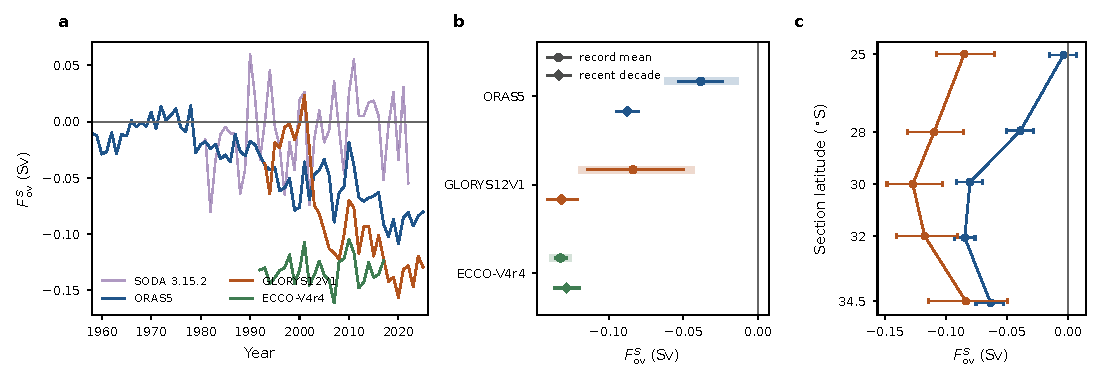
\includegraphics[width=\textwidth]{Fig1_sign.pdf}
  \caption{\textbf{The sign of the overturning freshwater transport at
  34.5\degS{}.}
  \textbf{a}, Annual-mean $\Fovs$. ORAS5, GLORYS12V1 and ECCO-V4r4 are computed
  here from monthly fields on the contiguous Atlantic section; SODA 3.15.2 is
  carried over from an annual-field pipeline, is not on the same basis, and is
  not used in any quantitative claim.
  \textbf{b}, Record mean (circles) and most recent decade (diamonds) with 95\%
  circular block-bootstrap intervals, at a 5-year block for the record mean and
  a 3-year block for the decade. The pale bar spans the intervals obtained for
  block lengths of 2 to 20 years. Between-product spread is 0.094~Sv, wider than
  the widest of these intervals (0.073~Sv, GLORYS12V1 across block lengths) and
  1.5 times the 5-year intervals quoted in the text.
  \textbf{c}, Mean $\Fovs$ over 1993--2025 against section latitude, with the
  same intervals. The open marker is the one case whose interval includes zero.}
  \label{fig:sign}
\end{figure}

\begin{figure}[t]
  \centering
  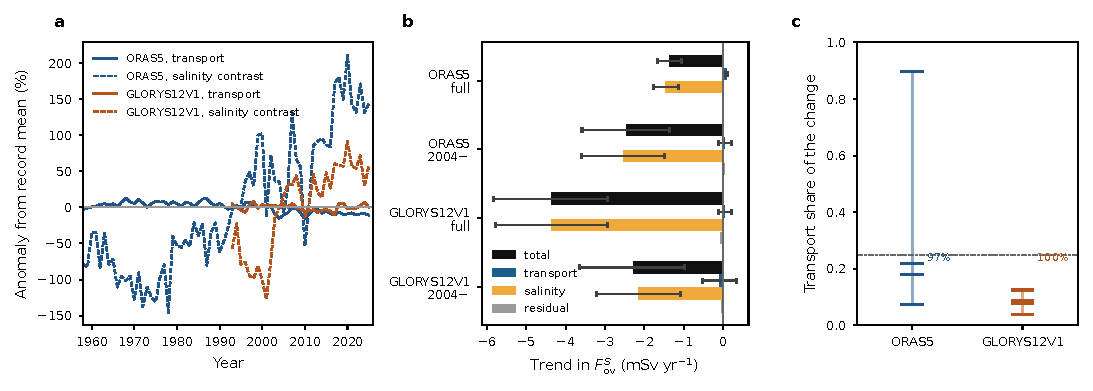
\includegraphics[width=\textwidth]{Fig2_attribution.pdf}
  \caption{\textbf{The decline is carried by the salinity contrast, not by the
  transport.}
  \textbf{a}, The two factors of equation~\eqref{eq:factorisation}, each as a
  percentage anomaly from its own record mean, so that a factor which barely
  moves can be compared with one that moves a great deal. The ORAS5 contrast
  passes close to zero early in the record, which is why its percentage anomaly
  is large there.
  \textbf{b}, Trend in $\Fovs$ split into transport and salinity contributions
  with 95\% block-bootstrap intervals, and the covariance residual, over each
  product's own record and over the Argo era.
  \textbf{c}, Transport share of the change over every non-overlapping epoch
  pair the record supports (2901 for ORAS5, 151 for GLORYS12V1) at epoch lengths
  of 10, 13 and 15 years, treated as a sensitivity analysis over window choice.
  Ticks mark the median, 90th and 95th percentiles and the maximum; the
  percentage is the fraction of pairs below the dashed 0.25 line.}
  \label{fig:attribution}
\end{figure}

\begin{figure}[t]
  \centering
  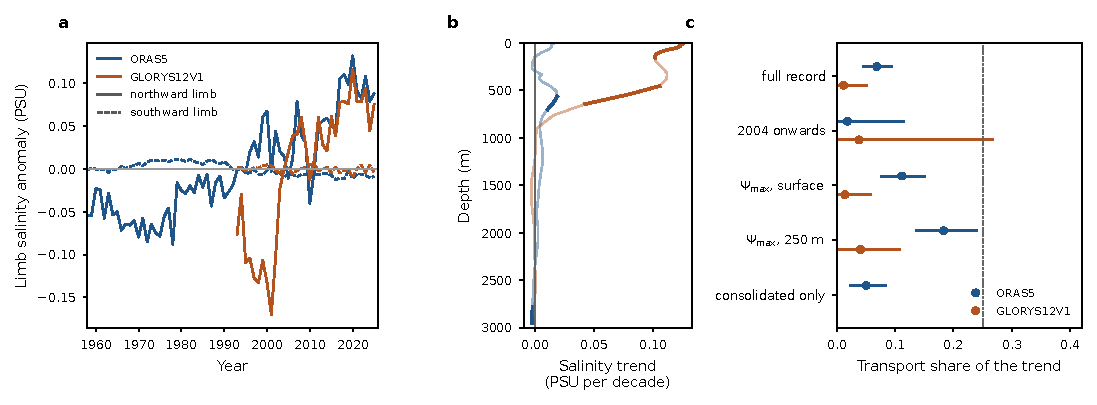
\includegraphics[width=\textwidth]{Fig3_mechanism.pdf}
  \caption{\textbf{The northward limb salinifies; the southward limb does not.}
  \textbf{a}, Transport-weighted salinity of the northward limb (solid) and the
  southward limb (dashed), as anomalies from their record means.
  \textbf{b}, Zonal-mean salinity trend against depth at the section over
  1993--2025, drawn bold where the pointwise Santer-adjusted $p$ is below 0.05.
  The panel is truncated at 3000~m; the abyssal limb discussed in the text
  begins below 4000~m.
  Adjacent levels are strongly correlated, so no field-significance claim is
  made from this panel.
  \textbf{c}, Transport share of the $\Fovs$ trend under every robustness test,
  with 95\% block-bootstrap intervals: the full record, the Argo era, two
  alternative definitions of the overturning strength, and, for ORAS5, the
  homogeneous consolidated stream alone.}
  \label{fig:mechanism}
\end{figure}

\begin{figure}[t]
  \centering
  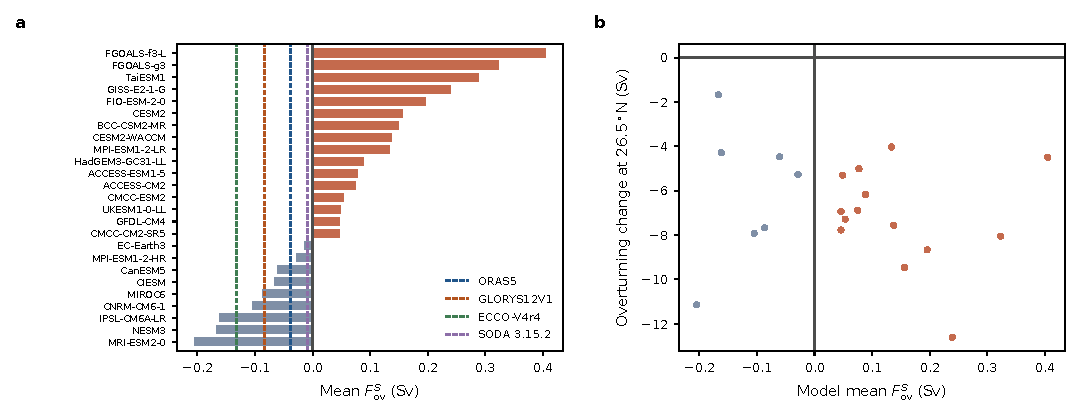
\includegraphics[width=\textwidth]{Fig4_models.pdf}
  \caption{\textbf{CMIP6 lies above the observational estimates, but cannot be
  sorted by the sign of $\Fovs$.}
  \textbf{a}, Mean $\Fovs$ at 34.5\degS{} over 1950--1980 in 25 CMIP6 models,
  with the reanalysis estimates marked; SODA is shown for continuity with
  Fig.~\ref{fig:sign} and is not used quantitatively. No offset or bias
  correction is applied to either models or reanalyses.
  \textbf{b}, Model mean $\Fovs$ against the overturning change at 26.5\degN{}
  from 1850--1900 to 2081--2100 in the 21 models with historical plus ssp585
  projections ($r=-0.20$, $p=0.40$, smallest reachable $|r|=0.43$). This
  replaces a 19-year single-member trend test, whose null result is guaranteed
  by internal variability: 19-year trends span $-3.5$ to $+2.4$~Sv per decade
  across 50 members of the MPI-ESM1-2-LR large ensemble.}
  \label{fig:models}
\end{figure}

\section*{Discussion}

Two statements about $\Fovs$ have been run together, and they need to be
separated. The first is that the Atlantic freshwater budget at 34.5\degS{} sits
on the side where the salt-advection feedback is self-reinforcing. Three
reanalyses spanning two ocean models and three assimilation methods agree on
that, with intervals clear of zero at every block length we tried, at every
latitude from 28 to 34.5\degS{} in the two products run on the latitude ladder, and in the most recent decade of each record.
The second is that the observed decline in $\Fovs$ measures a weakening
overturning. That statement does not survive contact with the same data.

The reason is a rate comparison rather than a ratio. In the two products that
decline, $\Fovs$ is changing at 36\% and 52\% of its own magnitude per decade
while the volume transport that carries it changes at 2.6\% and 0.6\%. Passed
through equation~\eqref{eq:factorisation} this makes the transport contribution
between 1\% and 18\% of the trend depending on how the overturning is defined
and over which window, with individual intervals reaching 27\%, and in most
configurations it has the opposite sign to the total. It is a minority
contribution under every test we ran in which the share is identified, though it
is not definition-independent:
it rises systematically as the definition of the overturning narrows from the
whole northward limb to the streamfunction maximum. Studies that read a falling
$\Fovs$ as a proxy for AMOC weakening, including the early-warning arguments
built on the $\Fovs$ minimum\cite{vanWesten2024} and an earlier, unpublished
version of our own analysis of these data, have attributed to the circulation a
change that the circulation did not make.

What did make it is a widening of the salinity contrast between the limbs,
carried by the northward limb while the southward limb does not change. How much
of that is a water-mass change rather than a redistribution of transport in
depth differs between products: in GLORYS12V1 it is 94\%, in ORAS5 only about
two thirds, with the salinity-only part there not individually significant. The
coarse upper-to-abyssal redistribution is small in both, and excluding the
abyssal cell makes the salinification larger rather than smaller, so what
remains in ORAS5 is a rearrangement of transport within the upper limb.

The part of this that observations can check, they support. Holding the
circulation fixed and letting only the EN4 objective analysis vary, the
northward limb salinifies at $+0.026$ to $+0.028$~PSU per decade
($p\le0.0005$) while the southward limb is flat. The limb asymmetry is
therefore present in a salinity field that no model integrates forward, and the
same construction returns a negative $\Fovs$, $-0.080$ to $-0.128$~Sv, from
observed salinity. The rate is less secure: ORAS5 runs about twice the
observation-only value over the same years while GLORYS12V1 is within 30\% of
it, and part of that gap is expected because EN4 relaxes to climatology where
profiles are sparse. The direction should be trusted; the ORAS5 rate should
not.
It also reframes what the diagnostic is sensing. A salinifying upper limb widens
the limb contrast and drives $\Fovs$ downward regardless of what the overturning
does, which is why $\Fovs$ and the transport are so weakly coupled on the
timescales the records resolve. It is consistent in direction with the South
Atlantic salinity accumulation attributed to a weakening
overturning\cite{Zhu2020,Zhu2023}, but our decomposition locates the change in
the transport-weighted upper limb rather than in the surface field, and we find
no transport change to accompany it.

Two things temper this. The first is that $\Fovs$ is not the freshwater budget
of the basin. The azonal component at this section is several times larger, of
the opposite sign, and trending upward by more than $\Fovs$ is trending
downward: significantly so in ORAS5, and marginally in GLORYS12V1 ($p=0.049$ on
8.5 effective degrees of freedom). Whether the basin as a whole is
moving deeper into the self-reinforcing regime is therefore not settled by
$\Fovs$ alone, and we make no claim that it is. Nor do we evaluate the northern
boundary: the indicator in the theory we cite is the freshwater convergence
between the southern and northern boundaries, and $\Fovs$ is a proxy for it
whose adequacy we have not tested. Both are natural next steps and neither is
addressed here.

The second is ECCO-V4r4, and it is a genuine disagreement rather than a caveat.
It is the only product here that is dynamically consistent by construction and
therefore the only one whose freshwater budget closes without assimilation
increments, and it shows no decline in $\Fovs$. Its limb salinities are flat only in the
aggregate: its upper cell salinifies at $+0.022$~PSU per decade ($p=0.025$),
the same sign as the other two products, while a significant redistribution
towards its abyssal cell cancels the effect. Against GLORYS12V1 this is
not an underpowered null: on the window the two share, ECCO's minimum detectable
limb-salinity trend of 0.020~PSU per decade is well below the GLORYS12V1 rate of
$+0.083$, so ECCO could have seen that salinification and did not. Against
ORAS5, whose common-window rate is $+0.019$, the comparison is inconclusive.
ECCO is also the one product in which the coarse limb redistribution is
significant and acts to cancel a positive water-mass term, so its flat limb
salinity is a cancellation rather than an absence of change. The mechanism we report is therefore a
property of the two sequential-assimilation products, and it remains possible
that what they are tracking is the arrival of the Argo array rather than a
change in the ocean. The evidence against that reading is that the attribution
is unchanged in every window and under every inhomogeneity correction we tried,
and that EN4 reproduces the limb asymmetry independently. The evidence for it is
that both sequential-assimilation products step at an observing-system boundary:
GLORYS12V1's decline is a level shift at the 2004 Argo transition rather than a
trend, and the ORAS5 record steps across its consolidated-to-operational join,
significantly so in the limb salinity itself ($+0.038$~PSU, $p=0.029$), after
which its Argo-era trend is no longer significant. Neither product's \emph{rate}
of decline should be taken at face value. We could not obtain the salinity
assimilation increments that would settle the question directly, and we regard
it as open.

Beyond that, all of these products are forced by the ERA family, so
cross-product agreement is a weaker form of independence than the product count
suggests: they differ in ocean model and in assimilation scheme, but not in the
atmosphere driving them. The Copernicus distribution of ORAS5 publishes one of
the system's five ensemble members\cite{Zuo2019}, so cross-product spread has to
stand in for within-product spread throughout, and that spread, 0.094~Sv, exceeds even the
widest within-product interval\cite{Jackson2019}. We compute
ECCO on the distributed 0.5\degree{} interpolation rather than the native LLC90
grid, which does not conserve transport exactly, and since ECCO is now the
load-bearing counterexample that limitation matters more than it would if it
were one supporting vote among four. The three products differ by 46\% in northward-limb transport
at this section (14.6 to 21.3~Sv), and we have not applied a published SAMBA or
SAMOC mean to arbitrate between them. That omission is not neutral: the weakest
of the three is ECCO, which is also our counterexample, so a comparison against
the observed mean transport could as easily undermine the counterexample as
support it, and it should be done before these numbers are used to weigh one
product against another. The reanalyses are also least
constrained by observations exactly where we evaluate them, since the observing
network at 34.5\degS{} is far sparser than the sustained array at
26.5\degN{}\cite{Meinen2018,Cunningham2007,GarzoliMatano2011,FrajkaWilliams2019}.

For models the implication cuts two ways. Correcting the freshwater transport
bias is necessary if a model is to represent the salt-advection feedback with
the right sign, and the CMIP6 median sits above every observational estimate we
computed. But the majority count usually quoted is not distinguishable from a
coin flip once model genealogy is accounted for, and we find no detectable
relationship between the sign of $\Fovs$ and the rate at which a model's
overturning weakens, either over the satellite era or over the forced response
to 2100, with a sample that could not have detected a moderate one. What we do
find is that model $\Fovs$ is strongly correlated with pre-industrial
overturning strength, which suggests that the freshwater transport bias is
partly a symptom of the overturning strength bias. If that is right, correcting
$\Fovs$ in isolation is the wrong target, and the two biases should be
addressed together.

What would settle the transient question is observational rather than
analytical. The claim we make is now a claim about limb salinities, which
sustained hydrography at 34.5\degS{} and the repeat sections that cross it can
test directly, without passing through an assimilating model; projecting an
observation-only salinity analysis onto the same limb mask is the single most
informative next step and we regard it as the test this result should be judged
by. Sustained transport monitoring at this latitude, extended towards the length
RAPID has reached at 26.5\degN{}, would constrain both factors of
equation~\eqref{eq:factorisation} at once. Reanalyses forced outside the ERA
family would test how much of the present agreement comes from shared boundary
conditions, and release of all five ORAS5 ensemble members would separate
assimilation noise from ocean signal within a single product. Until then the
defensible statement is the narrow one: the Atlantic freshwater budget sits
where the salt-advection feedback is self-reinforcing, and in the products that
decline, the recent decline in that diagnostic records a salinifying upper limb
rather than a slowing circulation.


\bibliographystyle{naturemag}
\bibliography{references}

\clearpage
\section*{Methods}

\subsection*{Ocean reanalyses}

Three reanalyses are computed here from monthly fields (Extended Data
Table~1). ORAS5\cite{Zuo2019} is a NEMO configuration at 0.25\degree{} with 75
vertical levels, assimilated by NEMOVAR 3D-Var FGAT and forced by ERA-40,
ERA-Interim and ERA5; we use 816 gap-free monthly fields of meridional velocity
and salinity covering 1958--2025. The Copernicus distribution joins the
consolidated reanalysis, which ends in 2014, to the operational stream
thereafter, and the two are treated separately wherever it matters.
GLORYS12V1\cite{JeanMichel2021} is a NEMO configuration at 1/12\degree{} with 50
levels, assimilated by a reduced-order Kalman filter and forced by ERA-Interim
and ERA5; we use 396 monthly fields covering 1993--2025. ECCO-V4r4\cite{Forget2015}
is an MITgcm state estimate on the LLC90 grid, nominally 1\degree{}, fitted to
observations by the adjoint method and therefore dynamically consistent by
construction, with no assimilation increments; its atmospheric forcing is
ERA-Interim plus estimated control adjustments. We analyse the distributed
0.5\degree{} lat-lon interpolation with 50 levels, using all 312 monthly fields
covering 1992--2017. Interpolation from the native grid does not conserve volume
transport exactly, which is a limitation we state rather than correct.

SODA 3.15.2\cite{Carton2018} is shown in Fig.~\ref{fig:sign}a for context but is
not used in any quantitative claim. It is a MOM5 and SIS configuration run at
1/4\degree{}, assimilated by optimal interpolation with bias correction and
forced by ERA5, and the archive we can obtain provides annual rather than
monthly fields on a regridded 0.5\degree{} Mercator grid. Because $\Fovs$ is
bilinear in velocity and salinity, forming it from annual means omits the
within-year covariance; measured in ECCO, where both routes are available, the
omission shifts $\Fovs$ by $+0.0124$~Sv, exceeding SODA's record mean of
$-0.0091$~Sv in magnitude. The corresponding shifts are $+0.0000$~Sv in ORAS5
and $-0.0013$~Sv in GLORYS12V1.

\subsection*{The section}

At the grid row nearest 34.5\degS{},
\begin{equation}
\Fovs \;=\; -\frac{1}{S_0}\int_{-H}^{0} V_{bc}(z)\,\big[\bar{S}(z)-S_0\big]\,\mathrm{d}z,
\label{eq:fovs}
\end{equation}
where $V_{bc}(z)$ is the zonally integrated meridional velocity after removal of
the net section transport, $\bar{S}(z)$ the width-weighted zonally averaged
salinity and $S_0=35$~PSU. A negative $\Fovs$ means the overturning imports
freshwater, equivalently that it exports salt from the Atlantic.

The Atlantic segment at each row is the contiguous run of ocean points
containing 25\degW{}, rather than a fixed longitude box. This matters. A box
from 70\degW{} to 20\degE{} at 34.5\degS{} admits, in GLORYS12V1, a second water
body of about 20 grid points near 58 to 57\degW{} whose surface salinity is
0.00 to 0.04~PSU. Those values are too fresh for the outer R\'io de la Plata,
which is brackish rather than fresh, so they are most likely estuary, lake or
land-mask cells rather than a resolved plume; either way they are not part of the
open Atlantic along this row. Including them depresses $\bar{S}$ in the upper
cells and shifts $\Fovs$ by $+0.013$~Sv, about a sixth of the GLORYS12V1 record
mean. At the 0.5\degree{} resolution of ECCO the feature is unresolved and the
contiguity test makes no difference. The resulting sections contain 294 ocean
points at 34.56\degS{} in ORAS5, 881 at 34.50\degS{} in GLORYS12V1 and 146 at
34.75\degS{} in ECCO; these are counts of ocean points, not of the width of a
longitude box.

The net transport removed is $-1.22$~Sv in ORAS5, $-1.17$ in GLORYS12V1 and
$-0.98$ in ECCO, and removing it shifts $\Fovs$ by $+0.0086$, $+0.0083$ and
$+0.0066$~Sv. It is of the sign and order expected for the Bering Strait inflow
plus net precipitation minus evaporation over the basin to the north, but we do
not claim it is that quantity: across the latitude ladder it varies
non-monotonically by 1.1~Sv in ORAS5 and 2.5~Sv in GLORYS12V1, far more than the
precipitation minus evaporation of the intervening bands, so a substantial part
of it is section construction, grid metrics or genuine mass imbalance. The
justification for removing it is that an overturning component of the freshwater
transport is not defined without doing so, and that equation~\eqref{eq:fovs} is
otherwise sensitive to $S_0$.

The azonal component is
$F_{az}=-(1/S_0)\iint v'S'\,\mathrm{d}x\,\mathrm{d}z$, with primes the
departures from the width-weighted zonal mean at each depth. It is computed from
monthly means and therefore excludes sub-monthly covariance.

\subsection*{The limb factorisation}

Because $\int V_{bc}\,\mathrm{d}z=0$, the depth levels where $V_{bc}>0$ carry a
volume transport $T$ exactly balanced by $-T$ in the levels where $V_{bc}<0$.
Defining the transport-weighted limb salinities
\begin{equation}
S_{\uparrow}=\frac{1}{T}\int_{V_{bc}>0}\! V_{bc}\bar{S}\,\mathrm{d}z,
\qquad
S_{\downarrow}=\frac{1}{T}\int_{V_{bc}<0}\! (-V_{bc})\bar{S}\,\mathrm{d}z,
\end{equation}
equation~\eqref{eq:fovs} becomes $\Fovs=-T(S_{\uparrow}-S_{\downarrow})/S_0$
exactly, because the $-S_0$ term integrates to zero. Both factors are computed
directly from the section profile and neither is defined in terms of the other,
which is what distinguishes this from writing $\Fovs=-\Psi\,\Delta_v S/S_0$
with $\Delta_v S\equiv-S_0\Fovs/\Psi$. In that construction the second factor is
the first divided out; it absorbs every change in the vertical structure of the
velocity as well as every change in salinity, it closes to machine precision by
construction, and the implied overturning share is fixed by the algebraic
identity
$(\Psi\text{ term})/\Delta\Fovs=(F_{\mathrm{early}}/\Delta\Fovs)\,(\delta\Psi/\Psi_{\mathrm{early}})$,
where $F_{\mathrm{early}}$ and $\Psi_{\mathrm{early}}$ are the base-epoch
values. We do not use it except as a labelled sensitivity test, and we note that
because that construction pins the share to the ratio of fractional changes it
cannot return a large value whatever the physics. The residual of the limb
factorisation is below $1.5\times10^{-14}$~Sv, which is double-precision
round-off and confirms only that the net transport removal closed.

\subsection*{Attribution}

For a change between two epochs we use the symmetric decomposition
\begin{equation}
\Delta\Fovs \;=\; -\frac{1}{S_0}\Big(\overline{\Delta S}\,\Delta T
\;+\; \overline{T}\,\Delta(\Delta S)\Big),
\label{eq:symmetric}
\end{equation}
with $\overline{T}$ and $\overline{\Delta S}$ the means of the two epochs. This
is exact, has no cross term to assign, and does not depend on which epoch is
taken as the base point. The asymmetric early-base and late-base expansions
differ from it by plus and minus half the cross term and are reported alongside.

The primary attribution is time-continuous. Holding one factor at its record
mean gives two counterfactual series, $F_T(t)=-T(t)\overline{\Delta S}/S_0$ and
$F_{\Delta S}(t)=-\overline{T}\,\Delta S(t)/S_0$. Unlike
equation~\eqref{eq:symmetric} this split is \emph{not} exact: the trends of the
two counterfactuals differ from the $\Fovs$ trend by the trend of the
transport-salinity covariance, and that residual is reported for every case in
the Results and in Fig.~\ref{fig:attribution}b. It is 3\% of the transport term
in ORAS5 over its own record and 108\% in GLORYS12V1, so for GLORYS12V1 the
transport contribution is quoted as not distinguishable from zero rather than as
a point value. The transport share is
$|{\rm trend}(F_T)|/|{\rm trend}(\Fovs)|$, quoted only where the total trend is
resolvable, because a ratio with an unresolved denominator is not identified.
The numerator and denominator are bootstrapped jointly, using the same block
indices, so the ratio interval is coherent. Two cases are excluded by that rule
and reported here for completeness: the ORAS5 common-window share is 0.368
[0.093, 6.19], and the ECCO census yields one usable pair out of 29.

The epoch census evaluates equation~\eqref{eq:symmetric} for every
non-overlapping early and late epoch pair a record supports at epoch lengths of
10, 13 and 15 years, discarding pairs whose total change is below 5~mSv in
magnitude, and reports the distribution of shares. These pairs are overlapping
views of one series, not independent samples, and are used as a sensitivity
analysis over window choice.

The overturning strength is also computed as the maximum of the depth-space
overturning streamfunction, from the surface and with the integration restarted
at 250~m, and the attribution repeated with each. Those streamfunctions are
cumulated from the uncorrected velocity, so that definition is independent of
how the net section transport is removed.

\subsection*{Limb composition}

The sign of $V_{bc}$ changes more than once, so the northward limb comprises an
upper cell and, beneath the southward deep water, a northward abyssal cell.
Writing $S_{\uparrow}=\sum_i w_i S_i$ over these sub-limbs with weights
$w_i=T_i/T$ summing to one, holding the weights at their record means isolates
the water-mass change and holding the sub-limb salinities at theirs isolates the
redistribution, exactly as in the main attribution. The decomposition is evaluated on monthly fields, so the
sub-limb transports sum to the same $T$ used elsewhere. The reconstructed
$S_{\uparrow}$ trend, $+0.027$~PSU per decade in ORAS5, still differs by about
7\% from the directly computed $+0.025$, because a mean of monthly products is
not the product of monthly means. Identifying the
sub-limbs on annual-mean profiles instead smooths out the deep sign reversals,
understates the abyssal cell by 26 to 30\% and leaves a shortfall against $T$ of
5.4\%, 4.1\% and 1.5\%; that route is not used. Vertical cell thicknesses are taken from
each product's own grid bounds rather than from differences of the cell-centre
depths, which for ECCO differ by 228~m in the column total.

Independently, the section is truncated at the deep zero crossing so that the
abyssal cell is excluded, the net-transport removal is re-applied within the
truncated layer so that the factorisation is again exact, and $\Fovs$, $T$ and
$\Delta S$ are recomputed for the upper cell alone.

\subsection*{Frozen-field and observation-only tests}

$\Delta S$ is transport-weighted, so it responds both to the salinity field and
to a redistribution of transport in depth. The two are separated by recomputing
the limb salinities with $\bar{S}(z)$ frozen at its record mean while
$V_{bc}(z,t)$ varies, and again with $V_{bc}(z)$ frozen while $\bar{S}(z,t)$
varies. This is done at the full vertical resolution of the section, so it
captures redistribution within a limb as well as between limbs. The sub-limb
decomposition described above resolves only the coarse upper-to-abyssal part and
is reported alongside it; it is evaluated on monthly fields so that the sub-limb
transports sum to the same $T$ used elsewhere.

For the observation-only test the velocity structure is frozen at each
reanalysis record-mean profile, interpolated onto the EN4.2.2 levels and
renormalised so that its depth integral again vanishes, and the limb salinities
are formed from the EN4 objective analysis of profile observations (g10
corrections) over 2005--2024, on a contiguous section built the same way. EN4 is
an optimal interpolation of profiles onto a 1\degree{} grid with no forward
model, so a trend computed this way is a trend in observed water masses under a
fixed circulation. Because EN4 is on whole-degree latitudes we use the
34\degS{} row: 34.5\degS{} rounds to 35\degS{}, which lies south of Cape
Agulhas (34.83\degS{}), where Africa no longer closes the basin and a
contiguous section runs east across the Indian Ocean to Australia. EN4 relaxes
towards climatology where profiles are sparse and core Argo does not sample
below 2000~m, so its trends are lower bounds.

\subsection*{Sensitivity to the removal of the net transport}

Because the limb split depends on where $V_{bc}$ changes sign, and that depends
on how the net section transport is removed, the whole analysis is repeated with
the net transport removed in proportion to $|V|$ rather than uniformly over the
cross-sectional area. $T$ changes by less than 0.6\% and the transport share by
less than 0.01 in both eddy-permitting products.

\subsection*{Statistics}

Trends are ordinary least squares on annual means. Significance uses the
effective sample size of Santer et al.\cite{Santer2000}: with $r_1$ the lag-1
autocorrelation of the regression residuals,
$N_{\text{eff}}=N(1-r_1)/(1+r_1)$, the slope standard error is inflated by
$\sqrt{(N-2)/(N_{\text{eff}}-2)}$ and the $t$-test uses $N_{\text{eff}}-2$
degrees of freedom. $N_{\text{eff}}$ is reported alongside adjusted
$p$-values in the Results, because several load-bearing tests have few
effective degrees of freedom; the GLORYS12V1 limb-salinity trend has
$N_{\text{eff}}=6.9$. For every window in which we report a null result we also
give the minimum detectable trend, the smallest slope that window could have
resolved at the 5\% level, so that an absence of significance is not read as an
absence of change. Correlation detection limits are quoted as the smallest $|r|$
reaching $p<0.05$, that is at 50\% power; the 80\% power thresholds are larger.

Trend confidence intervals come from a circular moving-block bootstrap of the
regression residuals with 10{,}000 iterations, added back to the fitted line and
refitted; resampling the values rather than the residuals would destroy the
trend and return a null distribution. Intervals on record means use a circular
moving-block bootstrap of the values, reported for block lengths of 2, 3, 5, 10,
15 and 20 years, with the 5-year value quoted in the text. Since a mean over a
trending record is not an estimate of a stationary population quantity, the mean
over the most recent decade is reported alongside it.

Where a record contains a known inhomogeneity, trends are refitted as
$F(t)=a+bt+c\,\mathrm{I}(t\ge t_{\text{splice}})$, with $\mathrm{I}$ the
indicator function, so that the level shift and
the trend are estimated jointly, with standard errors inflated by the same
Santer factor computed from the residuals of that fit. For ORAS5,
$t_{\text{splice}}=2015$. Estimating the step by differencing stream means
instead conflates it with the trend and gives a larger value, which is why the
regression estimate is the one quoted.

Per-depth salinity trends in Fig.~\ref{fig:mechanism}b are marked at the
pointwise 5\% level; adjacent levels are strongly correlated, so no
field-significance claim is made from them and none is used in the argument.

\subsection*{CMIP6 and observed transports}

Mean $\Fovs$ at 34.5\degS{} is computed for 25 CMIP6\cite{Eyring2016}
historical simulations over 1950--1980 on their native grids by
equation~\eqref{eq:fovs}, one realisation per model. No offset or bias
correction of any kind is applied, to either the models or the reanalyses. Model
genealogy is accounted for by grouping close relatives (CESM2 with CESM2-WACCM
and TaiESM1, the two MPI-ESM1-2 resolutions, the two ACCESS models, the two
FGOALS models, the two CMCC models, and UKESM1-0-LL with HadGEM3-GC31-LL) and
retaining the member whose $\Fovs$ is median within each family. Only the MPI
family is internally inconsistent in sign, and the count is reported for both of
its members. Sign counts are tested against a binomial null. Two provenances of the model
$\Fovs$ were in circulation in earlier work and differ by up to 0.041~Sv (root
mean square 0.016~Sv over 16 models, worst case MPI-ESM1-2-LR) without changing
any sign; everything here uses the decomposition summary alone.

Overturning at 26.5\degN{} is taken from \texttt{msftmz}, or \texttt{msftyz}
where \texttt{msftmz} is unavailable, on the \texttt{atlantic\_arctic\_ocean}
basin of the native \texttt{gn} grid for variant \texttt{r1i1p1f1}, as the maximum over depths at or below 500~m of annual means,
with historical and ssp585 concatenated. Trends over 2005--2023 are available
for 16 models and the change from 1850--1900 to 2081--2100 for 21. The
internal-variability floor for a 19-year trend is taken from 50 members of the
MPI-ESM1-2-LR large ensemble. Leave-one-out ranges are reported for all three
correlation tests.

The RAPID array\cite{Cunningham2007} gives $-0.889$~Sv per decade at
26.5\degN{} over 2005--2023, with an unadjusted $p$ of 0.093 that becomes 0.205
after the effective-sample-size correction ($N_{\text{eff}}=11.9$). We do not compare the modelled mean transports against
the SAMBA array at 34.5\degS{}\cite{Meinen2018,FrajkaWilliams2019}. The
relevant published quantity would be a mean rather than a trend, and its absence
here is a limitation rather than a consequence of the array's length.

\subsection*{Data availability}

ORAS5 is distributed by the Copernicus Climate Data Store, GLORYS12V1 by the
Copernicus Marine Service, ECCO-V4r4 by NASA PO.DAAC, SODA 3.15.2 by the
University of Maryland, RAPID by the RAPID-AMOC programme and CMIP6 output
through the Earth System Grid Federation. Dataset identifiers, version strings
and access dates are listed in the archived code repository.

\subsection*{Code availability}

Analysis and figure code is archived with the manuscript. The section profiles
and the limb factorisation are computed by
\texttt{compute\_paper3v2\_section\_profiles.py}, the attribution and its
robustness tests by \texttt{analysis\_paper3v2\_attribution.py}, the limb
composition by \texttt{analysis\_paper3v2\_limb\_composition.py}, the splice and
fractional-rate analysis by \texttt{analysis\_paper3v2\_stepfit.py}, the latitude
sensitivity by \texttt{analysis\_paper3v2\_latitude\_sensitivity.py}, the CMIP6
analysis by \texttt{analysis\_paper3v2\_cmip6.py}, and each figure by the
correspondingly named \texttt{plot\_paper3v2\_*.py} script.

\clearpage

\section*{Extended Data}

\begin{figure}[h]
  \centering
  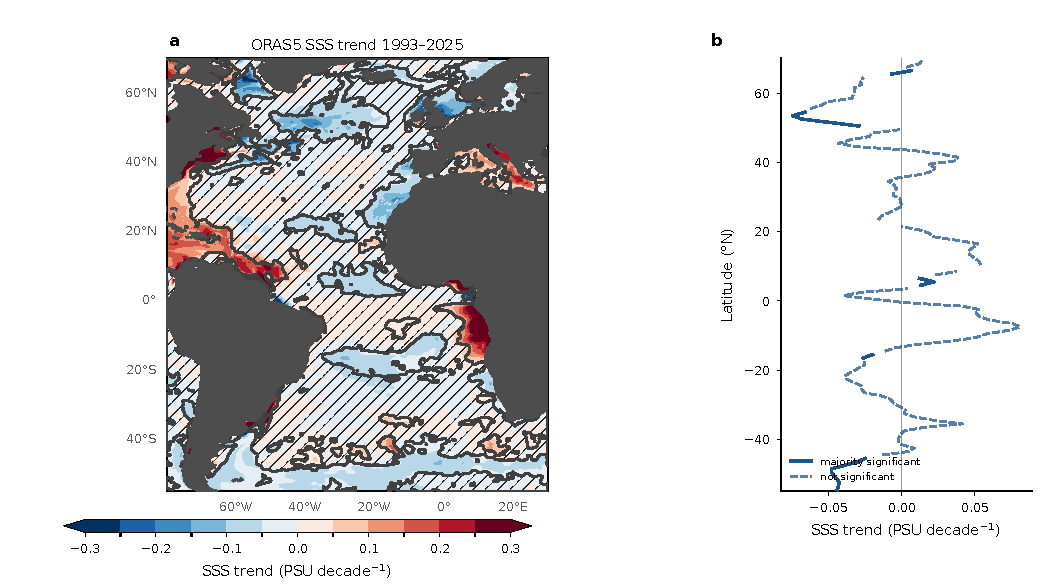
\includegraphics[width=0.94\textwidth]{../extended_data/ED1a_sss_trend_oras5.pdf}\\[0.4em]
  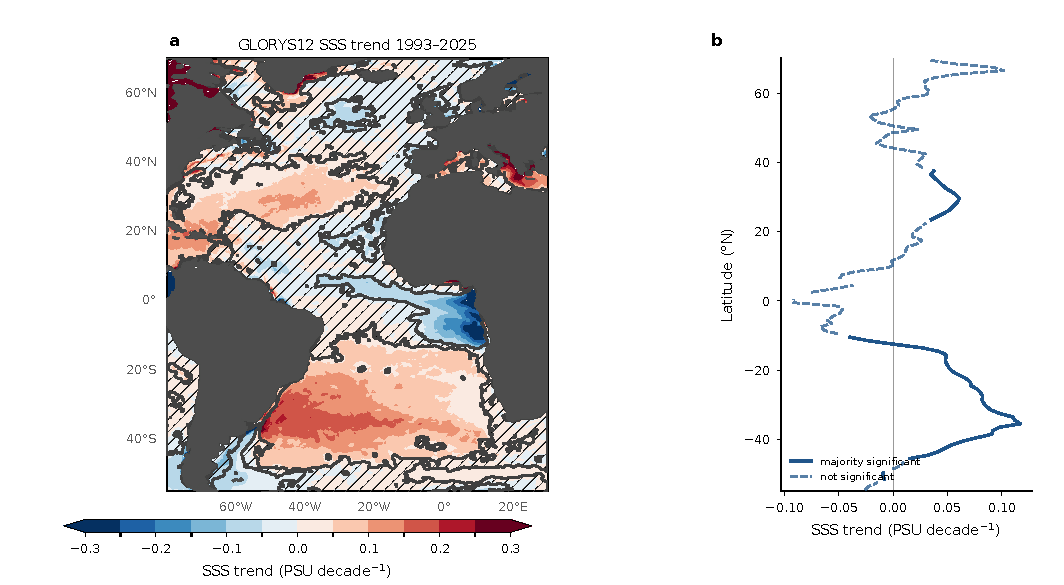
\includegraphics[width=0.94\textwidth]{../extended_data/ED1b_sss_trend_glorys12.pdf}
  \caption*{}
\end{figure}

\textbf{Extended Data Fig.~1 $\vert$ Surface salinity trends, 1993--2025.}
Per-pixel trends on deseasonalised monthly anomalies for ORAS5 and GLORYS12V1,
hatched where the Santer-adjusted $p$ exceeds 0.05. The effective-sample-size
correction reduces the significant ocean area from 76\% to 36\% in ORAS5 and
from 76\% to 51\% in GLORYS12V1. Atlantic band means disagree in sign between
the products in all three bands examined (60\degN{} to 80\degN{}, 40\degN{} to
60\degN{}, 10\degS{} to 35\degS{}), and only one of the six band-and-product
combinations is significant, GLORYS12V1 over 10\degS{} to 35\degS{}
($+0.061$~PSU per decade, $p=0.0002$). There is no significant subpolar North
Atlantic freshening in either product. Surface salinity trend patterns are in
any case ambiguous, since amplification of the water cycle and a uniform surface
heat flux both produce patterns resembling the one that would be attributed to
ocean transport\cite{Zika2018}, which is why the argument in the main text rests
on the transport-weighted limb salinities at the section and these maps are not
used as evidence.

\begin{figure}[h]
  \centering
  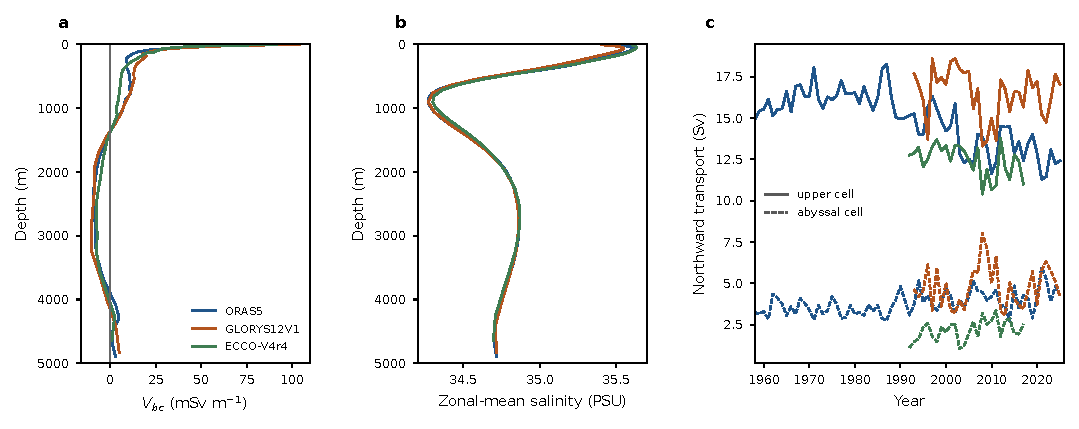
\includegraphics[width=0.98\textwidth]{../extended_data/ED2_section.pdf}
  \caption*{}
\end{figure}

\textbf{Extended Data Fig.~2 $\vert$ Section profiles and the structure of the
limbs.} \textbf{a}, Time-mean zonally integrated meridional velocity after
removal of the net section transport, over the matched 1993--2017 window. The
sign changes of this profile define the limbs. \textbf{b}, Time-mean zonally
averaged salinity over the same window. \textbf{c}, The northward-limb transport
split into its upper cell (solid) and its abyssal cell (dashed), on monthly
fields so that the two sum to $T$. The barotropic-corrected velocity changes sign
three to seven times in ORAS5 (modally four), three to four in GLORYS12V1 and
three to five in ECCO; the upper limb reaches to about 1325, 1245 and 1318~m
respectively, and the abyssal limb begins at about 4044, 4405 and 4264~m. The abyssal cell carries 3.8, 4.8 and 2.2~Sv, that is 20\%,
23\% and 15\% of the northward limb, and is 0.21 to 0.49~PSU fresher than the
upper cell, which is why the redistribution between them has to be excluded
before the widening contrast can be read as a water-mass change. Its transport trend
is significant in ECCO ($+0.36$~Sv per decade, $p=0.041$) and in ORAS5
($+0.17$, $p=0.0004$), and not in GLORYS12V1.

\textbf{Extended Data Table~1 $\vert$ Reanalysis products.}

\begin{center}
\small
\begin{tabular}{lllll}
\toprule
 & ORAS5 & GLORYS12V1 & ECCO-V4r4 & SODA 3.15.2 \\
\midrule
Ocean model        & NEMO & NEMO & MITgcm & MOM5, SIS \\
Model resolution   & 0.25$^\circ$ & 1/12$^\circ$ & LLC90, $\sim$1$^\circ$ & 0.25$^\circ$ \\
Grid analysed      & native & native & 0.5$^\circ$ lat-lon & 0.5$^\circ$ Mercator \\
Vertical levels    & 75 & 50 & 50 & 50 \\
Assimilation       & NEMOVAR 3D-Var & reduced-order & adjoint & optimal \\
                   & FGAT           & Kalman filter & (no increments) & interpolation \\
Atmospheric forcing & ERA-40, ERA-Interim, & ERA-Interim, & ERA-Interim & ERA5 \\
                    & ERA5 & ERA5 & (adjusted) & (COARE4) \\
Fields used        & 816 monthly & 396 monthly & 312 monthly & 43 annual \\
$T$, 1993--2017 (Sv) & 17.9 & 21.1 & 14.6 & not recomputed \\
Record             & 1958--2025 & 1993--2025 & 1992--2017 & 1980--2022 \\
Ocean points       & 294 & 881 & 146 & not recomputed \\
$T$ (Sv)           & 18.7 & 21.3 & 14.6 & not recomputed \\
$\Delta S$ (PSU)   & $+0.068$ & $+0.136$ & $+0.307$ & not recomputed \\
Used quantitatively & yes & yes & yes & no \\
\bottomrule
\end{tabular}
\end{center}


\end{document}
